% main_English.tex — compact version (target: 12 pages, Springer LNCS)
\documentclass[runningheads]{llncs}

\usepackage[T1]{fontenc}
\usepackage{graphicx}
\usepackage{subcaption}
\usepackage{amsmath}
\usepackage{booktabs}
\usepackage{multirow}
\usepackage{url}
\usepackage[section]{placeins}
\usepackage{float}

\graphicspath{{../assets/paper/}}

\begin{document}

%% ----------------------------------------------------------------
%%  TITLE & AUTHORS
%% ----------------------------------------------------------------
\title{Instance Segmentation, Not Semantics, Limits Individual Tree Detection in Dense ULS Point Clouds}

\author{Arturo~Cant\'u~Olivares\inst{1} \and
Diego~Sebastian~Cruz~Cervantes\inst{1} \and
Luis~Fernando~Maldonado\inst{1} \and
Jes\'us~Gabriel~Gudi\~no~Lara\inst{1} \and
Daniel Cant\'on~Enriquez\inst{1}}

\authorrunning{A.~Cant\'u~Olivares et al.}
\titlerunning{Instance Segmentation Limits Tree Detection in Dense ULS Point Clouds}

\institute{Universidad Aut\'onoma de Quer\'etaro (UAQ), Quer\'etaro, M\'exico\\
\email{dcruz54@alumnos.uaq.mx}}

\maketitle

%% ----------------------------------------------------------------
%%  ABSTRACT
%% ----------------------------------------------------------------
\begin{abstract}
Automated individual tree segmentation (ITS) in high-density UAV laser scanning (ULS) point clouds is critical for scalable forest inventories, yet it remains unclear whether semantic preprocessing or the instance segmentation step is the main performance bottleneck. We present a controlled factorial comparison ($3 \times 2$ design) of three preprocessing strategies --- no preprocessing, Random Forest (RF) on geometric features, and PointNet++ MSG --- combined with two variants of a volumetric Watershed~3D segmenter (classic CHM seeding and a novel density-based seeding), calibrated independently per pipeline and evaluated on the FOR-instance~V1 benchmark across five forest types. Despite near-perfect semantic quality (tree~IoU~$>$~0.97 for both classifiers), instance F1 peaks at 0.209, revealing that the instance segmenter --- not the semantic preprocessor --- is the dominant bottleneck. RF with geometric features outperforms PointNet++ MSG in all pipeline combinations without requiring a GPU, and density-based seeding consistently improves over CHM seeding (+47\% for RF, +74\% for PointNet++), particularly in dense uniform-height canopies where CHM is nearly flat.
\keywords{Individual Tree Segmentation \and UAV laser scanning (ULS) \and Semantic segmentation \and Watershed 3D \and Density seeding \and Random Forest \and PointNet++ \and FOR-instance}
\end{abstract}

%% ================================================================
%%  1. INTRODUCTION
%% ================================================================
\section{Introduction}\label{sec:intro}

\subsection{Motivation}

Automated forest inventories at the individual tree level are essential for carbon stock estimation, biodiversity monitoring, and precision forestry. UAV laser scanning (ULS) provides point densities one to two orders of magnitude higher than conventional ALS ($\sim$7{,}000~pts/m$^2$ vs.\ $\sim$5~pts/m$^2$), enabling characterization of individual trees including crowns, trunks, branches, and understory. However, automated Individual Tree Segmentation (ITS) in ULS data remains an open problem due to height model noise, crown--understory ambiguity, and structural variability across forest types.

ITS pipelines typically operate in two cascaded stages: a semantic classifier that isolates tree points from ground, understory and noise, followed by an instance segmenter that assigns each tree point to a unique tree identifier. Deep learning methods such as PointNet++~\cite{qi2017} have raised expectations for semantic quality, yet their practical advantage over classical Random Forest classifiers in the specific context of ITS preprocessing remains unclear. At the same time, 3D volumetric Watershed methods have evolved beyond the classical 2D CHM approach~\cite{dalponte2016}, enabling direct exploitation of vertical point density. Despite these advances, the relative impact of each stage on end-to-end performance has rarely been isolated experimentally~\cite{qi2017,breiman2001,puliti2023}, and no controlled study has systematically varied the preprocessor while keeping the instance segmenter identical across multiple forest types.

\subsection{Contributions}

The contributions of this work are: (1)~a factorial comparison $3 \times 2$ of three semantic preprocessors (no preprocessing, RF, PointNet++ MSG) $\times$ two seeding strategies (CHM, density) on FOR-instance~V1~\cite{puliti2023}, with independent per-pipeline calibration; (2)~evidence that the instance segmenter, not the preprocessor, is the dominant bottleneck; (3)~demonstration that RF without a GPU outperforms PointNet++ in all combinations; and (4)~a crown-density seeding variant that consistently improves over classic CHM seeding in uniform-height canopies.

%% ================================================================
%%  2. RELATED WORK
%% ================================================================
\section{Related Work}\label{sec:related}

\subsection{Individual tree detection and instance segmentation}

In conventional ALS (${<}10$~pts/m$^2$), the dominant ITS approach detects CHM local maxima and delineates crowns via 2D watershed~\cite{popescu2002,silva2016,dalponte2016}. These methods degrade in dense, multi-layered canopies where crowns overlap. ULS data (${\sim}10^3$--$10^4$~pts/m$^2$) enables volumetric 3D approaches that separate adjacent trunks and understory via fill rather than horizontal projection~\cite{dalponte2016}, but few works isolate the contribution of semantic preprocessing from the instance segmenter. This gap motivates our controlled factorial design.

\subsection{Semantic segmentation of forest point clouds}

Classical methods use handcrafted geometric features with Random Forest~\cite{breiman2001} or SVM~\cite{weinmann2015,weinmann2017}, while deep learning methods (PointNet~\cite{qi2016}, PointNet++~\cite{qi2017}) learn features end-to-end. PointNet++ has shown promising ULS results with height-normalized features, but semantic classification is predominantly evaluated as a final task; its role as ITS preprocessing remains understudied.

\subsection{Benchmarks}

FOR-instance~V1~\cite{puliti2023} assembles ULS plots from five forest types across four continents with point-level semantic and instance annotations. FOR-instanceV2~\cite{xiang2025} extends it; we evaluate on V1 for comparability. NeonTreeEvaluation~\cite{weinstein2021} provides multi-modal data but is limited to North American ecosystems.

%% ================================================================
%%  3. DATASET
%% ================================================================
\section{Dataset}\label{sec:dataset}

\subsection{FOR-instance}

FOR-instance~V1~\cite{puliti2023} is a ULS benchmark with point-level semantic and instance annotations. We use five of the six collections (Table~\ref{tab:collections}), excluding NIBIO2 to avoid over-representing Norwegian boreal forest, which would bias aggregated metrics. Point densities range from $454$ to $10{,}156$~pts/m$^2$ (per-collection median: RMIT~$473$, TUWIEN~$1{,}406$, CULS~$2{,}510$, SCION~$3{,}064$, NIBIO~$7{,}246$). Geographic and structural diversity is key: NIBIO accounts for 50\% of the test set (dense boreal forest), while RMIT and TUWIEN present radically different crown structures.

\begin{table}[H]
\centering
\caption{FOR-instance V1 collections used in this work.}\label{tab:collections}
\begin{tabular}{llccc}
\toprule
Code & Country & Forest type & Test plots & GT trees \\
\midrule
NIBIO  & Norway        & Boreal conifer (\emph{P.~abies})          & 6 & 161 \\
CULS   & Czech Rep.    & Temperate conifer (\emph{P.~sylvestris})  & 1 &  20 \\
TUWIEN & Austria       & Mixed alluvial deciduous                  & 1 &  35 \\
RMIT   & Australia     & Dry sclerophyll (eucalypts)               & 1 &  64 \\
SCION  & New Zealand   & Conifer plantation (\emph{P.~radiata})    & 2 &  43 \\
\midrule
\textbf{Total} & & & \textbf{11} & \textbf{323} \\
\bottomrule
\end{tabular}
\end{table}

\subsection{Splits and Reproducibility}\label{sec:splits}

We use the official split (70\% dev / 30\% test) with an internal train/val subdivision (80/20\%) at plot level with a fixed seed, following~\cite{henrich2024,wielgosz2024}.

%% ================================================================
%%  4. METHODOLOGY
%% ================================================================
\section{Methodology}\label{sec:method}

\subsection{Pipeline Overview}

All pipelines share a two-stage architecture: (1)~semantic preprocessing and (2)~a Watershed~3D instance segmenter, varied factorially across five pipelines (Fig.~\ref{fig:pipeline}). Segmenter parameters are independently calibrated per pipeline via grid search on the validation set (instance F1, IoU~3D~$\geq 0.5$).

\begin{figure}[H]
\centering
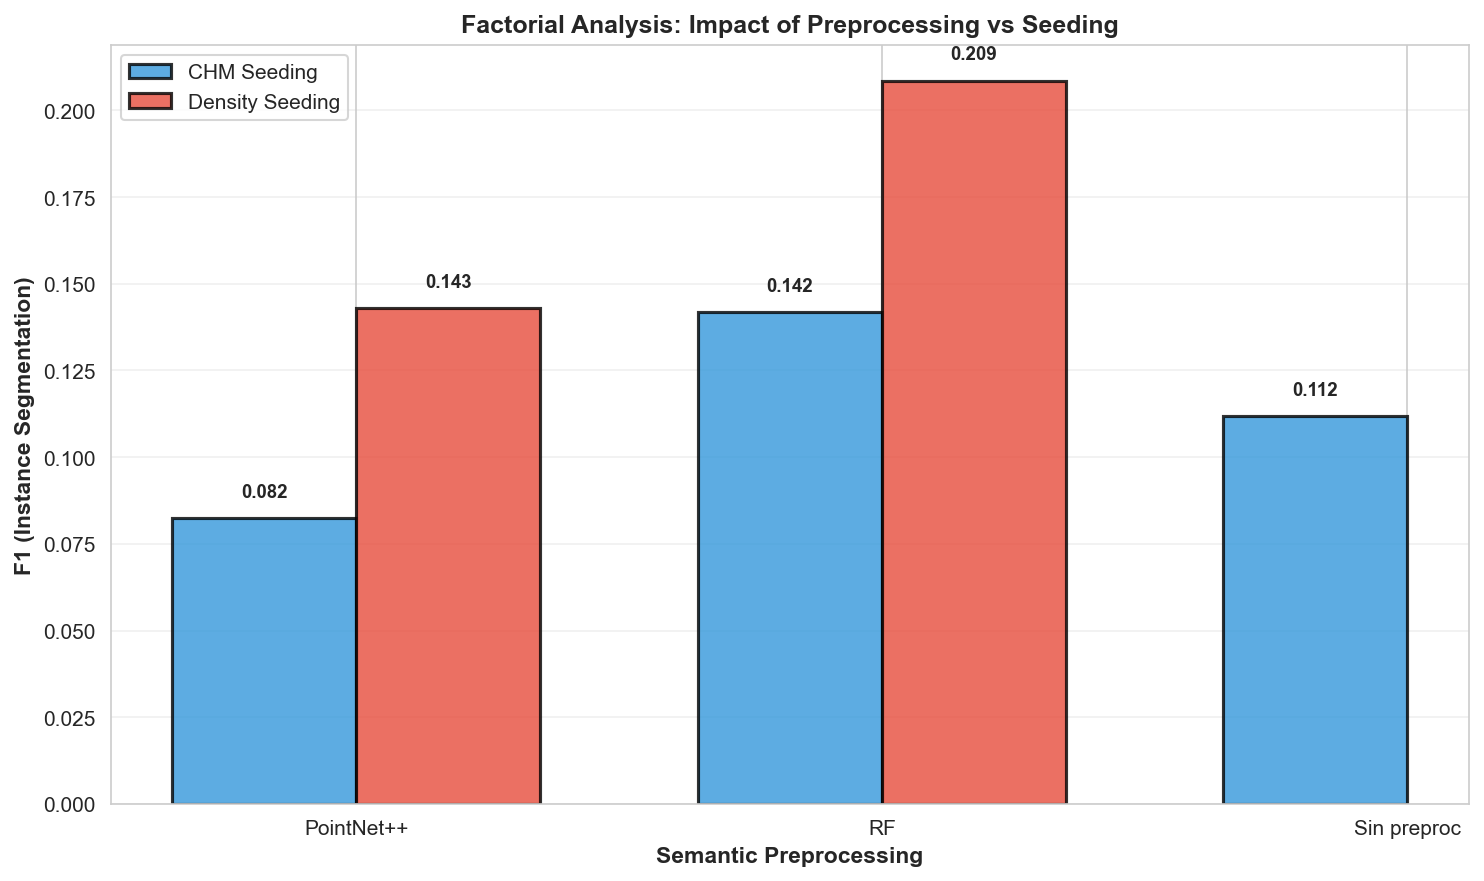
\includegraphics[width=\textwidth]{fig_05_factorial_analysis}
\caption{Factorial analysis: density-based seeding (red) outperforms CHM (blue) across all methods (+47--74\%), with a larger gain than switching the preprocessor (+27\%).}\label{fig:pipeline}
\end{figure}

\subsection{Pipeline~A --- No Preprocessing (Baseline)}

The full point cloud (excluding classes $\{0, 3\}$) is passed directly to the segmenter. All pipelines share HAG computation from a DTM interpolated over ground points, truncated to $[0, 50]$\,m.

\subsection{Pipeline~B --- Random Forest on Geometric Features}

Each point is represented by 27 geometric features: 8 eigen-based descriptors and 5 local descriptors (HAG, verticality, roughness, vertical range, normalized intensity), computed at two neighborhoods $k \in \{20, 50\}$, plus local volumetric density ($r = 0.5$\,m)~\cite{weinmann2015,weinmann2017}. A maximum search radius of $5.0$\,m is enforced. The classifier is a Random Forest ($n=200$ trees, class-balanced) trained with subsampling of $12{,}000$ pts/class/plot.

\subsection{Pipeline~C --- PointNet++ MSG}

We use PointNet++ MSG~\cite{qi2017} with four Set Abstraction and four Feature Propagation modules~\cite{yan2019pointnet2pytorch}. Input features are 5 dimensions per point ($XYZ$ + HAG\_norm + intensity), ensuring information equivalence with Pipeline~B. The network is trained for 100 epochs with subsamples of $8{,}192$ points. At inference, multiple passes are performed with probability averaging; residual points are labeled by KNN interpolation ($k=3$).

\subsection{Instance Segmenter --- Volumetric Watershed 3D}\label{sec:watershed}

The segmenter operates on points classified as tree in HAG and follows four steps: (1)~3D voxelization in $(X, Y, \text{HAG})$; (2)~3D Gaussian smoothing of the density grid; (3)~seed detection; and (4)~volumetric watershed on the inverted smoothed density with an occupied-voxel mask~\cite{dalponte2016}. Unlike 2D watershed on the CHM, volumetric fill correctly separates adjacent trunks and understory points.

\paragraph{CHM variant (Pipelines A, B, C).} Seeds are detected on the upper envelope of the volume (equivalent to a CHM derived from the 3D grid itself) via \texttt{peak\_local\_max}.

\paragraph{Density variant (Pipelines D, E).} The CHM is replaced by a density surface accumulated within a band of \emph{top\_band\_m} meters below the highest voxel in each column. This surface captures local point concentrations even when the CHM is nearly flat, as in dense boreal forests with uniform canopy height.

\paragraph{Calibration.}
Parameters are calibrated by independent per-pipeline grid search (Table~\ref{tab:grid-search}, Fig.~\ref{fig:gridsearch}).

\begin{table}[H]
\centering
\caption{Optimal Watershed~3D parameters per pipeline (grid search on val, instance F1, IoU~3D~$\geq 0.5$).}\label{tab:grid-search}
\resizebox{\textwidth}{!}{%
\begin{tabular}{lcccccc}
\toprule
Parameter & Search space & A & B (RF) & C (PN++) & D (RF+Dens.) & E (PN++Dens.) \\
\midrule
voxel\_size (m)         & $\{0.1, 0.2, 0.3\}$      & 0.2 & 0.1 & 0.1 & 0.2 & 0.3 \\
gaussian\_sigma         & $\{0.3, 0.5, 1.0\}$      & 0.3 & 0.3 & 1.0 & 0.5 & 0.3 \\
min\_crown\_radius\_m   & $\{0.5, 1.0, 1.5, 2.0\}$ & 0.5 & 1.0 & 1.5 & 2.0 & 1.5 \\
top\_band\_m            & $\{2.0, 3.0, 5.0\}$      & --- & --- & --- & 2.0 & 5.0 \\
\midrule
Mean val F1             &                           & 0.272 & 0.371 & 0.377 & 0.467 & 0.450 \\
\bottomrule
\end{tabular}%
}
\end{table}

\begin{figure}[H]
\centering
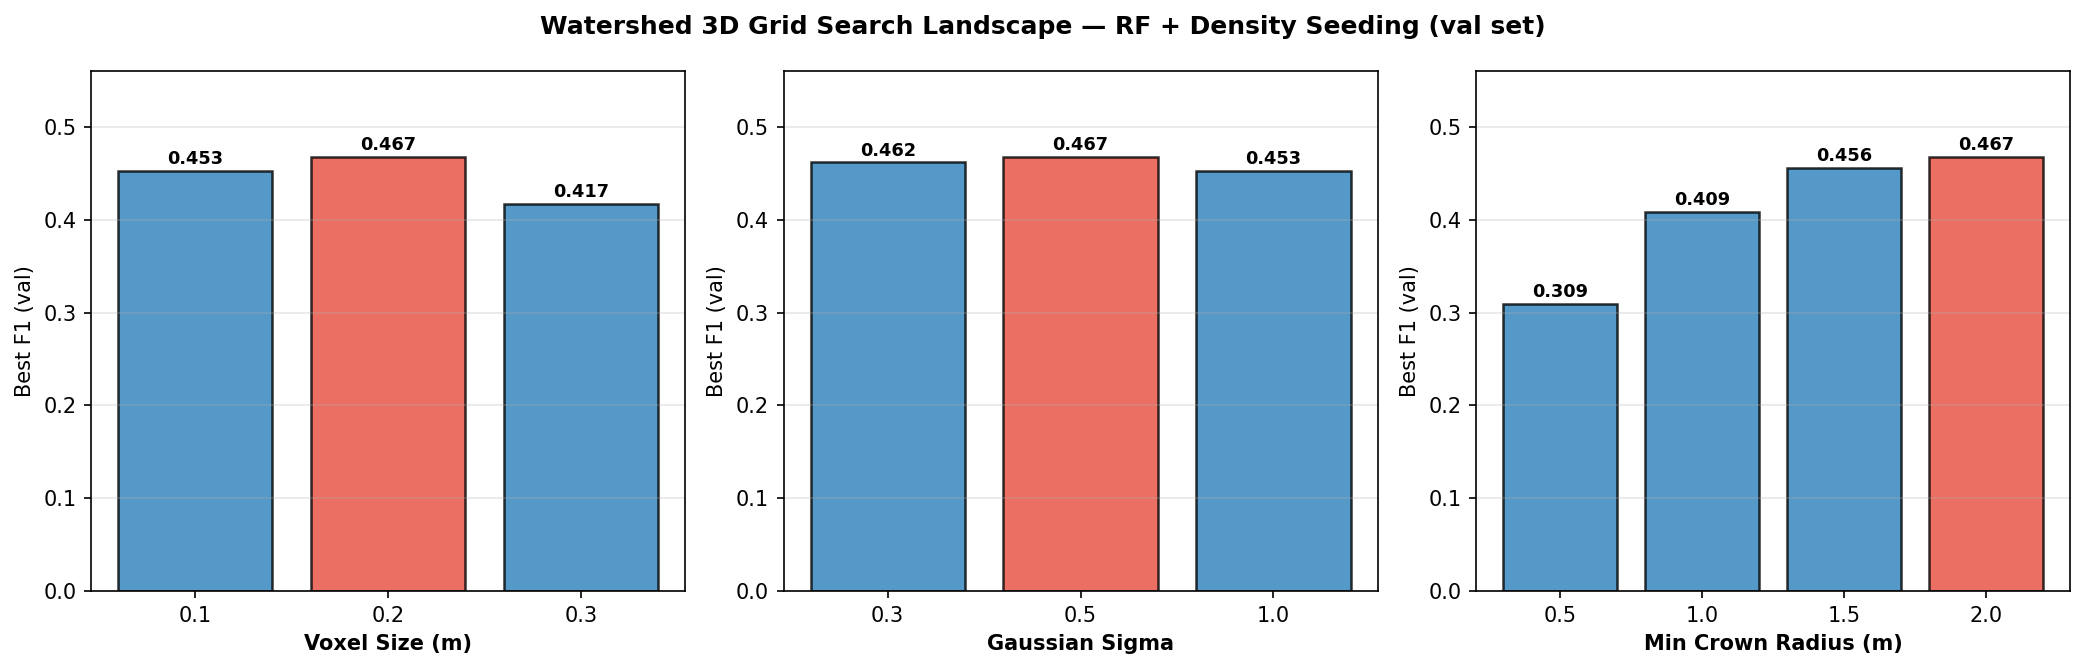
\includegraphics[width=\textwidth]{fig_v4_gridsearch_landscape}
\caption{Grid search landscape for Pipeline~D (RF + Density). Red bars: optimal value. Minimum crown radius (2.0\,m) is the most decisive parameter.}\label{fig:gridsearch}
\end{figure}

%% ================================================================
%%  5. EVALUATION PROTOCOL
%% ================================================================
\section{Evaluation Protocol}\label{sec:eval}

\textbf{Semantics.} We report tree~IoU ($TP/(TP+FP+FN)$), seg~mIoU (mean IoU over both classes), and binary seg~F1 (tree/non-tree) at point level.

\textbf{Instances.} Predicted instances $\{P_i\}$ are matched to GT instances $\{G_j\}$ via greedy matching by point-wise IoU~3D with threshold $\tau = 0.5$, following~\cite{henrich2024,wielgosz2024}:

\begin{equation}
\text{IoU}_{3D}(P_i, G_j) = \frac{|P_i \cap G_j|}{|P_i \cup G_j|}
\end{equation}

We compute precision, recall, F1, and \emph{coverage} (fraction of GT trees with at least one prediction with IoU$_{3D} \geq \tau$, without unique matching): the Coverage~$-$~Recall gap indicates crown fragmentation. Reporting both tasks allows us to isolate which stage concentrates the error.

%% ================================================================
%%  6. RESULTS
%% ================================================================
\section{Results}\label{sec:results}

\subsection{Aggregated Results}

Table~\ref{tab:results-agg} reports results on the test set. Pipeline~D (RF + Density) achieves the best instance F1 (0.209), outperforming Pipeline~B (RF + CHM, 0.142) by 47\% and the baseline (0.112) by 87\%. Density seeding consistently improves both methods: RF rises from 0.142 to 0.209 and PointNet++ from 0.082 to 0.143.

\begin{table}[H]
\centering
\caption{Aggregated results (test, IoU~3D~$\geq 0.5$, average over 11~plots).}\label{tab:results-agg}
\resizebox{\textwidth}{!}{%
\begin{tabular}{llccccccc}
\toprule
Pipeline & Seeding & sem mIoU & tree IoU & sem F1 & inst Prec & inst Recall & inst F1 & Coverage \\
\midrule
A --- No preproc.        & CHM     & --    & --    & --    & 0.138 & 0.133 & 0.112 & 0.133 \\
B --- Random Forest      & CHM     & 0.985 & 0.990 & 0.996 & 0.394 & 0.110 & 0.142 & 0.110 \\
C --- PointNet++ MSG     & CHM     & 0.974 & 0.982 & 0.994 & 0.172 & 0.060 & 0.082 & 0.060 \\
D --- Random Forest      & Density & 0.985 & 0.990 & 0.996 & 0.418 & 0.150 & \textbf{0.209} & 0.150 \\
E --- PointNet++ MSG     & Density & 0.974 & 0.982 & 0.994 & 0.209 & 0.118 & 0.143 & 0.118 \\
\bottomrule
\end{tabular}%
}
\end{table}

Both classifiers achieve tree~IoU~$>$~0.97, yet this quality does not translate proportionally into instance performance (peak F1 0.209), identifying the segmenter as the bottleneck.

\subsection{Results by Site}

Fig.~\ref{fig:semantic} shows the semantic classification on CULS~2. The key difference between classifiers is not the error volume ($<1\%$) but its distribution: RF produces crown-edge false positives, while PointNet++ generates isolated false positives on the ground that become spurious seeds.

\begin{figure}[H]
\centering
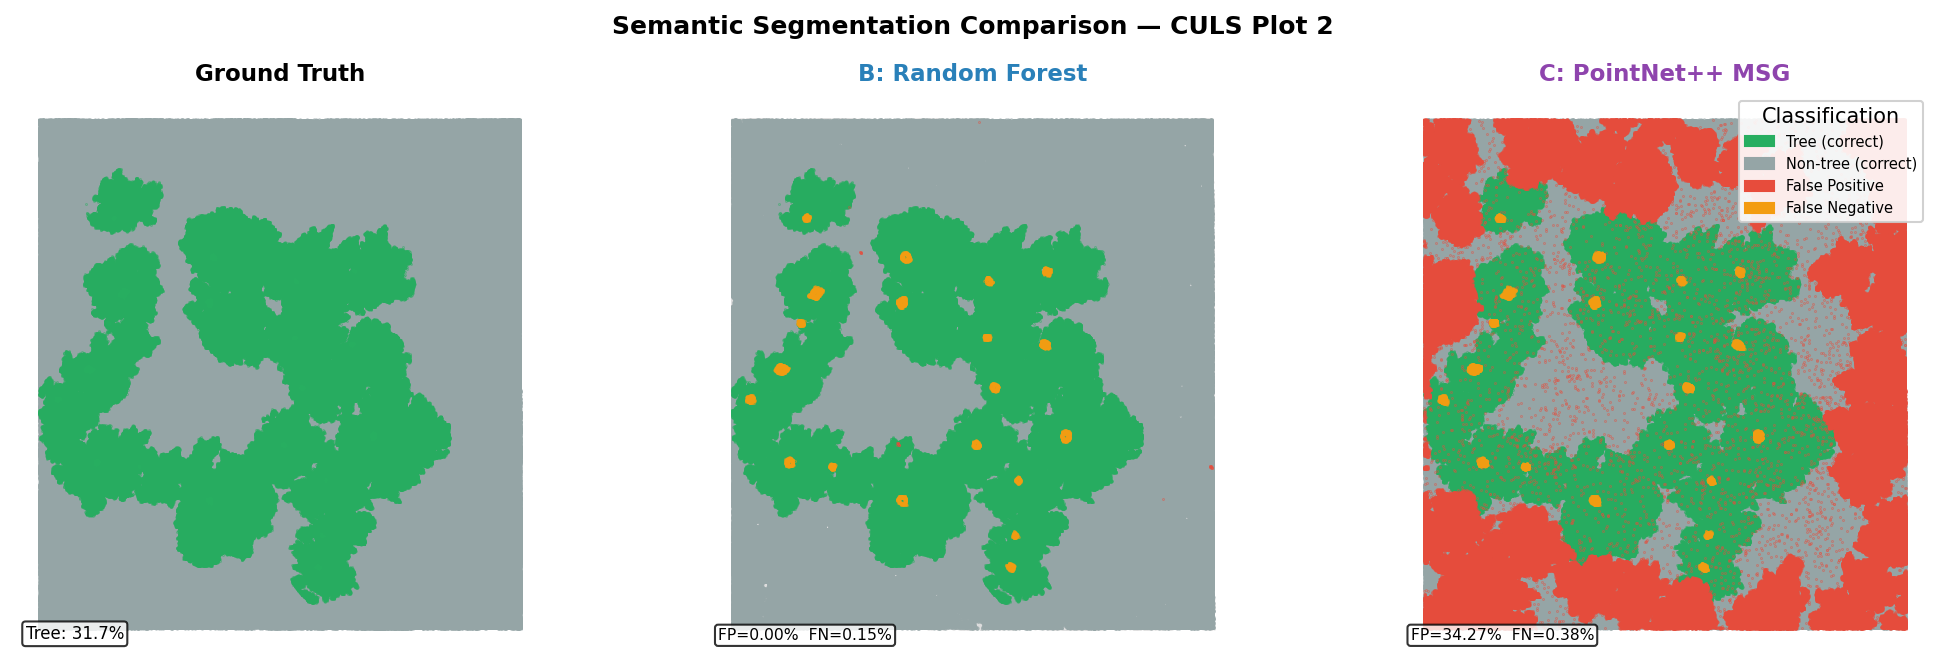
\includegraphics[width=\textwidth]{fig_v3_semantic_overlay}
\caption{Semantic classification on CULS~2. Green: correct tree; red: FP; orange: FN. RF concentrates errors at crown edges; PointNet++ produces isolated FPs on the ground.}\label{fig:semantic}
\end{figure}

Fig.~\ref{fig:f1site} shows per-site F1. Key patterns: (i)~CULS is the only site with F1~$>$~0.5, thanks to well-separated crowns; (ii)~NIBIO (50\% of the test set) is the most challenging case due to its dense, uniform canopy; (iii)~density seeding improves across all sites, with the largest relative gain in RMIT (RF: 0.061$\to$0.213) and TUWIEN (RF: 0.000$\to$0.136), where CHM is particularly ineffective.

\begin{figure}[H]
\centering
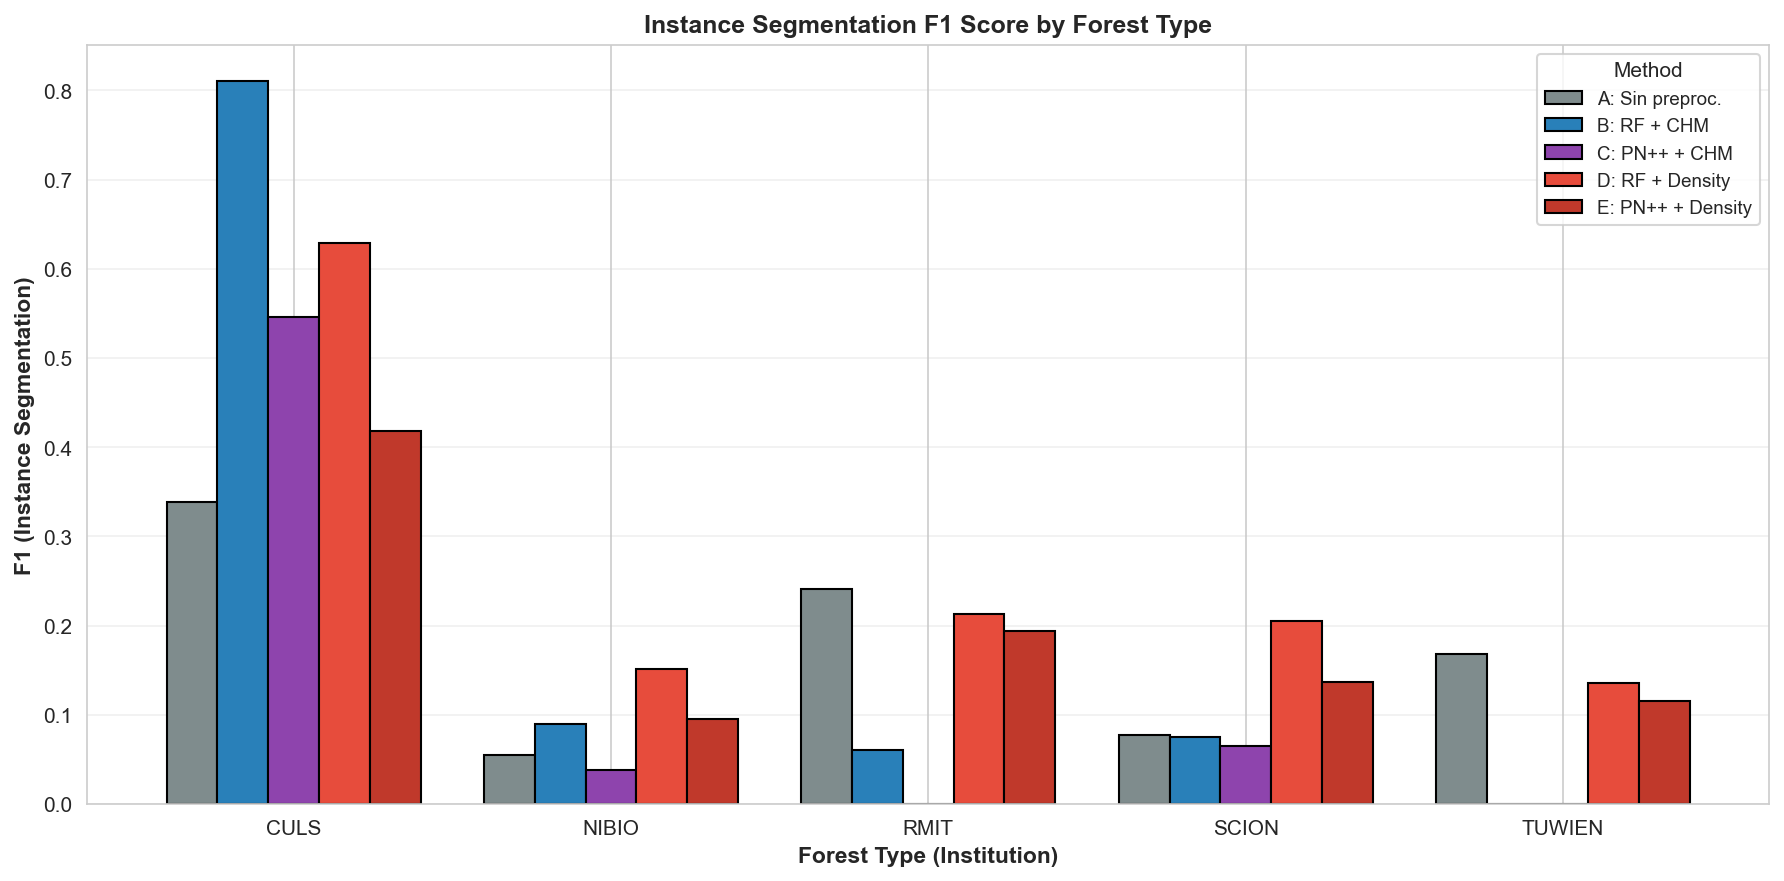
\includegraphics[width=\textwidth]{fig_02_f1_by_institution}
\caption{Instance F1 by forest type. Pipeline~D (RF + Density, red) leads at all sites except CULS (F1\,=\,0.811 with Pipeline~B).}\label{fig:f1site}
\end{figure}

\subsection{Instance Segmentation Visualizations}

Figs.~\ref{fig:topculs} and~\ref{fig:topnibio} show top-view predictions: CULS exhibits good crown separation while NIBIO shows persistent over-merging.

\begin{figure}[H]
\centering
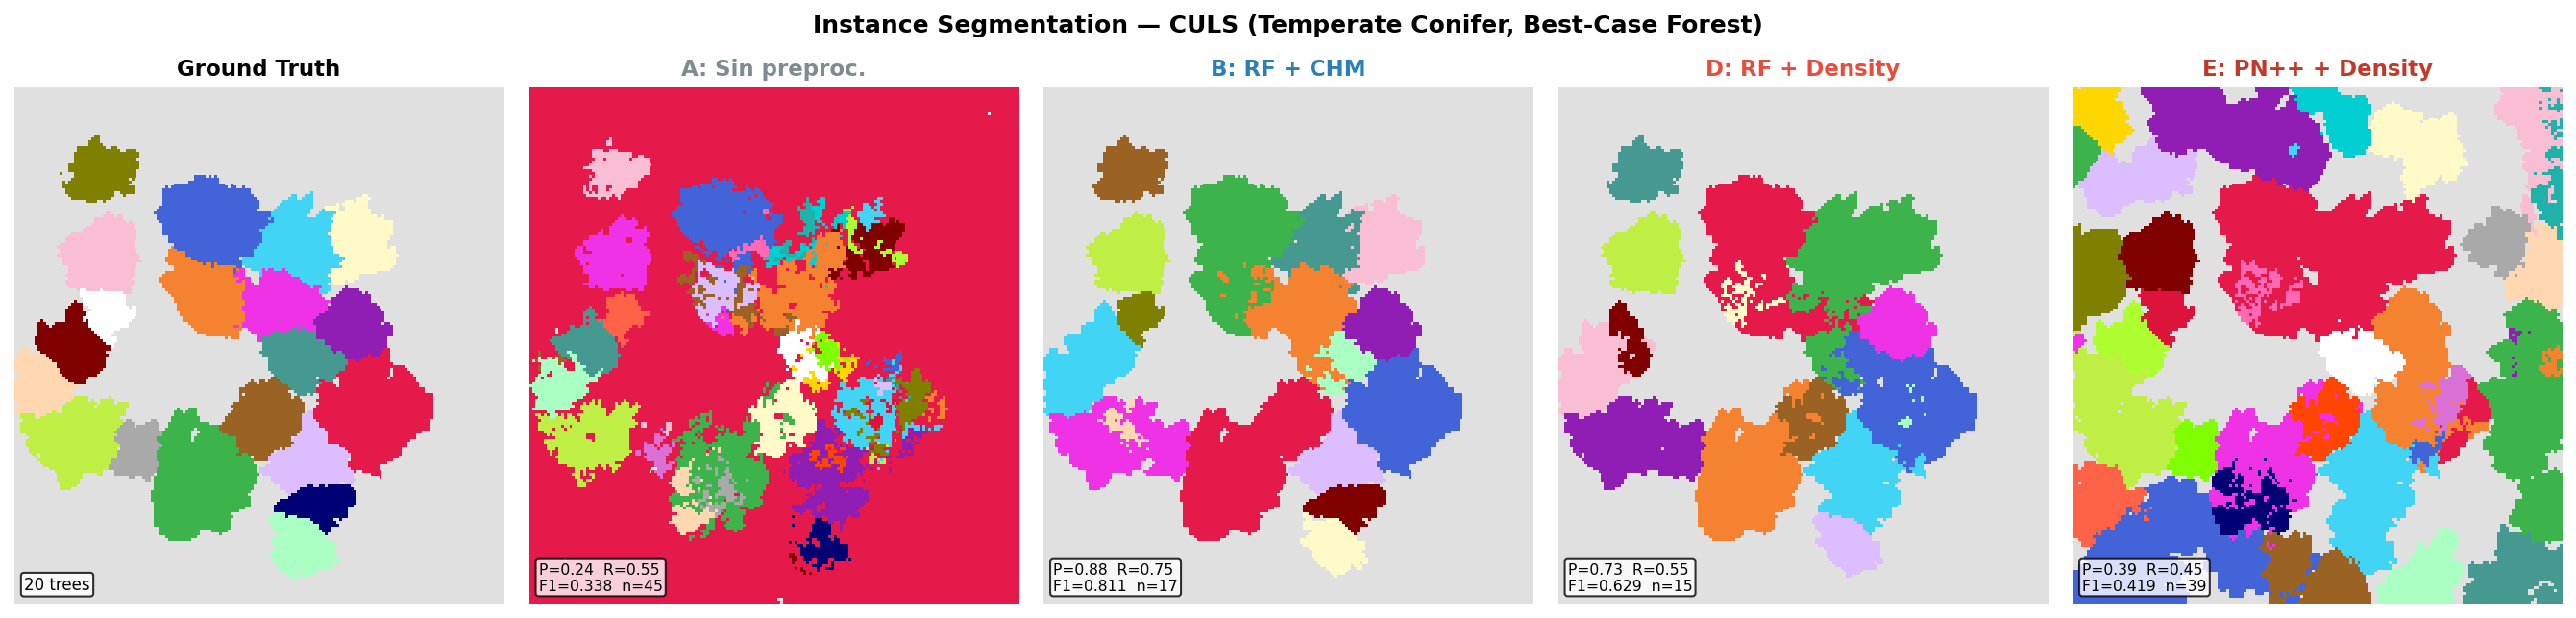
\includegraphics[width=\textwidth]{fig_v1_topview_culs}
\caption{Top view of CULS~2. Pipeline~D achieves the best separation (F1\,=\,0.629); CHM seeding tends to merge adjacent crowns.}\label{fig:topculs}
\end{figure}

\begin{figure}[H]
\centering
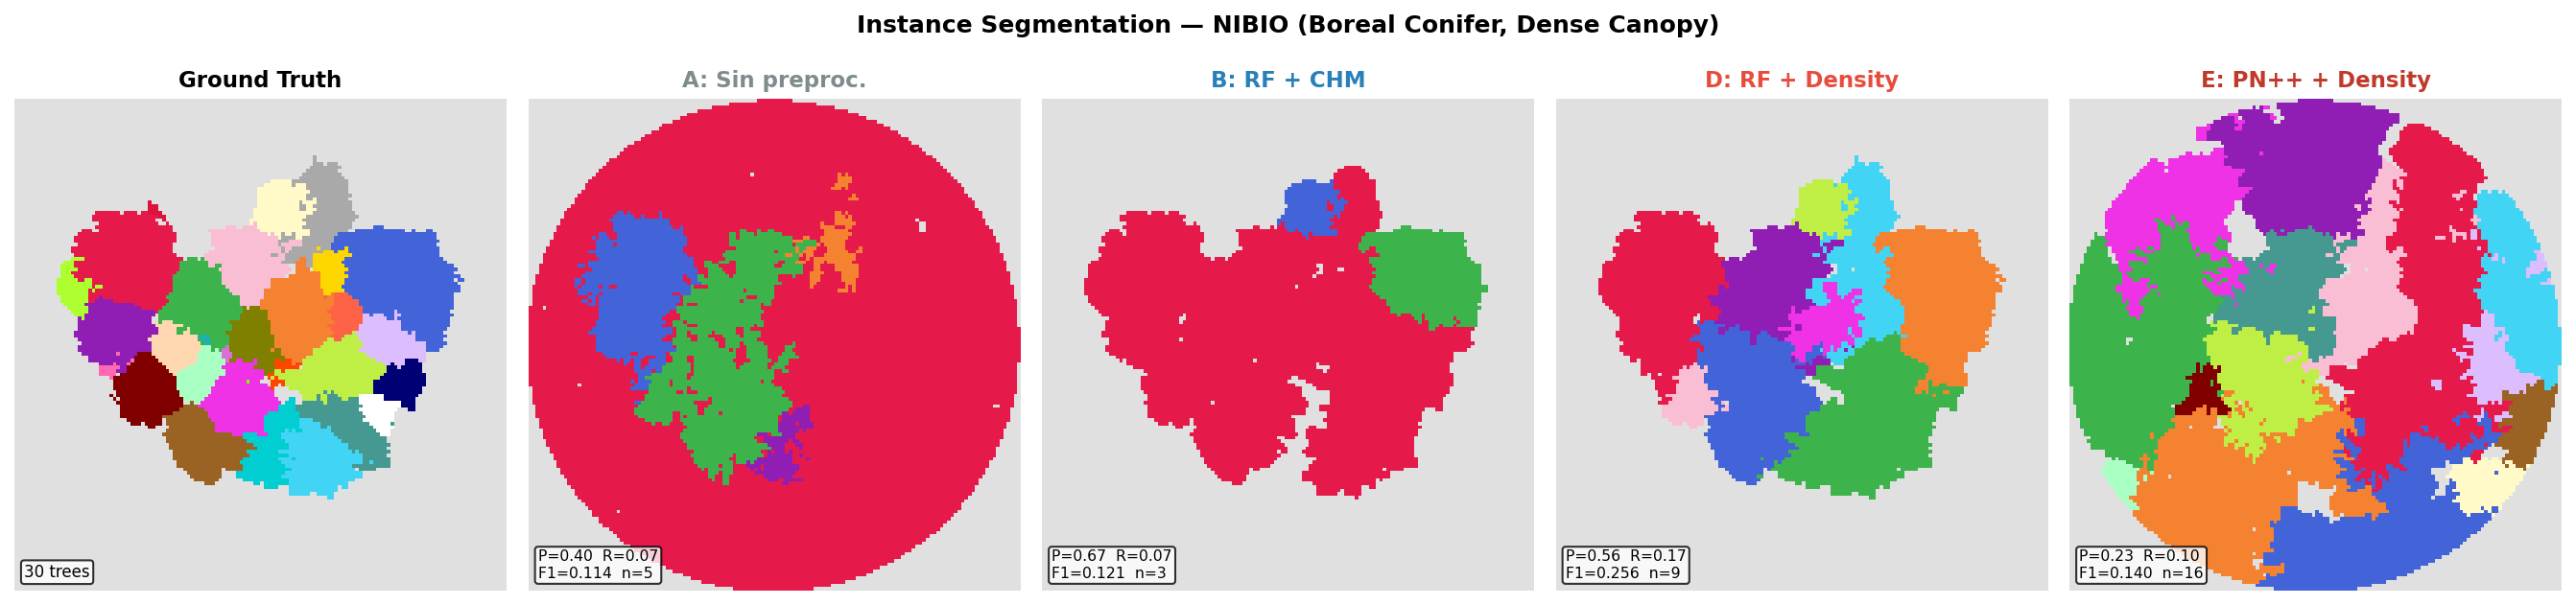
\includegraphics[width=\textwidth]{fig_v2_topview_nibio}
\caption{Top view of NIBIO~17 (dense boreal). Severe under-segmentation across all methods; maximum F1 0.256 with Pipeline~D.}\label{fig:topnibio}
\end{figure}

\subsection{Factorial Analysis: Preprocessor $\times$ Seeding}

\begin{table}[H]
\centering
\caption{Instance F1 (test) in the factorial design. $\Delta$: relative improvement of Density seeding over CHM.}\label{tab:factorial}
\begin{tabular}{lccc}
\toprule
Preprocessor & CHM & Density & $\Delta$ \\
\midrule
No preproc.\ (baseline) & 0.112 & ---   & ---   \\
Random Forest           & 0.142 & \textbf{0.209} & +47\% \\
PointNet++ MSG          & 0.082 & 0.143 & +74\% \\
\bottomrule
\end{tabular}
\end{table}

The factorial analysis (Table~\ref{tab:factorial}, Fig.~\ref{fig:decoupling}) confirms that switching seeding strategy (CHM $\rightarrow$ Density) yields a larger improvement (+47--74\%) than switching the preprocessor (baseline $\rightarrow$ RF, +27\%), identifying the segmenter as the dominant bottleneck. The interaction between both factors is relevant: the cleaner semantics of RF produce fewer spurious seeds, resulting in lower over-segmentation (Precision RF+Density: 0.418 vs.\ PN++Density: 0.209).

\begin{figure}[H]
\centering
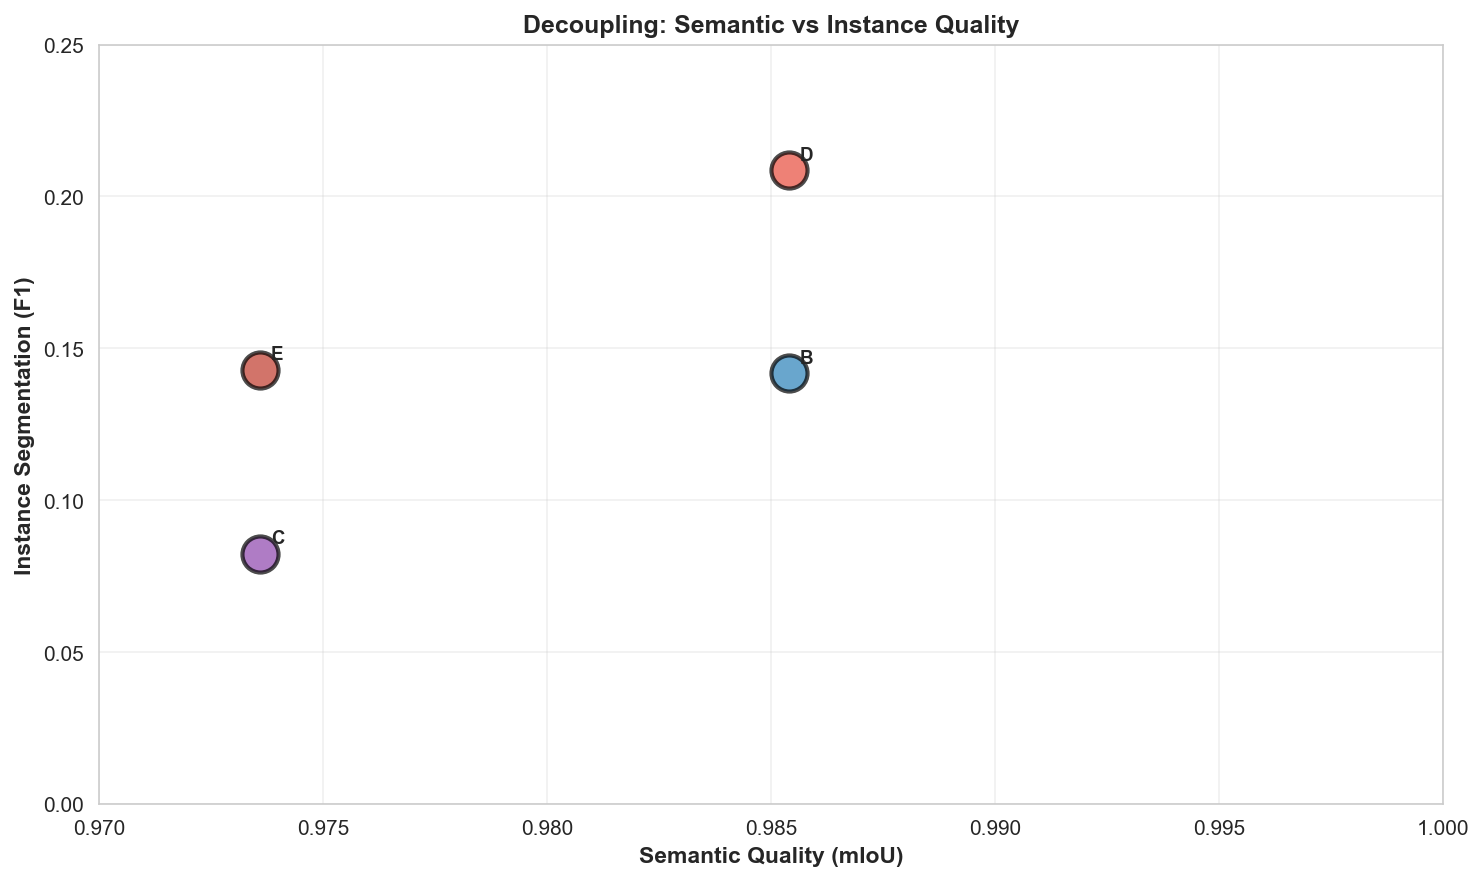
\includegraphics[width=\textwidth]{fig_03_semantic_instance_decoupling}
\caption{Semantic--instance decoupling. Tree~IoU~$>$~0.97 for both classifiers, yet instance F1 differs by $2.5\times$ (RF vs.\ PN++ with CHM). The segmenter is the dominant factor.}\label{fig:decoupling}
\end{figure}

\subsection{Feature Importance --- Random Forest}

HAG dominates RF classification with 61.5\% of cumulative Gini importance across its two scales ($k\!=\!50$: 0.325; $k\!=\!20$: 0.290), confirming that height above ground is the primary predictor for tree/non-tree separation. Verticality (0.087) and roughness (0.072) at coarse scale provide complementary geometric information.

%% ================================================================
%%  7. DISCUSSION
%% ================================================================
\section{Discussion}\label{sec:discussion}

\subsection{The Segmenter as the Bottleneck}

Fig.~\ref{fig:vprofile} illustrates how Pipeline~D correctly assigns trunk and branch points in CULS~2, whereas a 2D CHM projection would conflate these points. The volumetric fill of Watershed~3D is the decisive structural difference.

\begin{figure}[H]
\centering
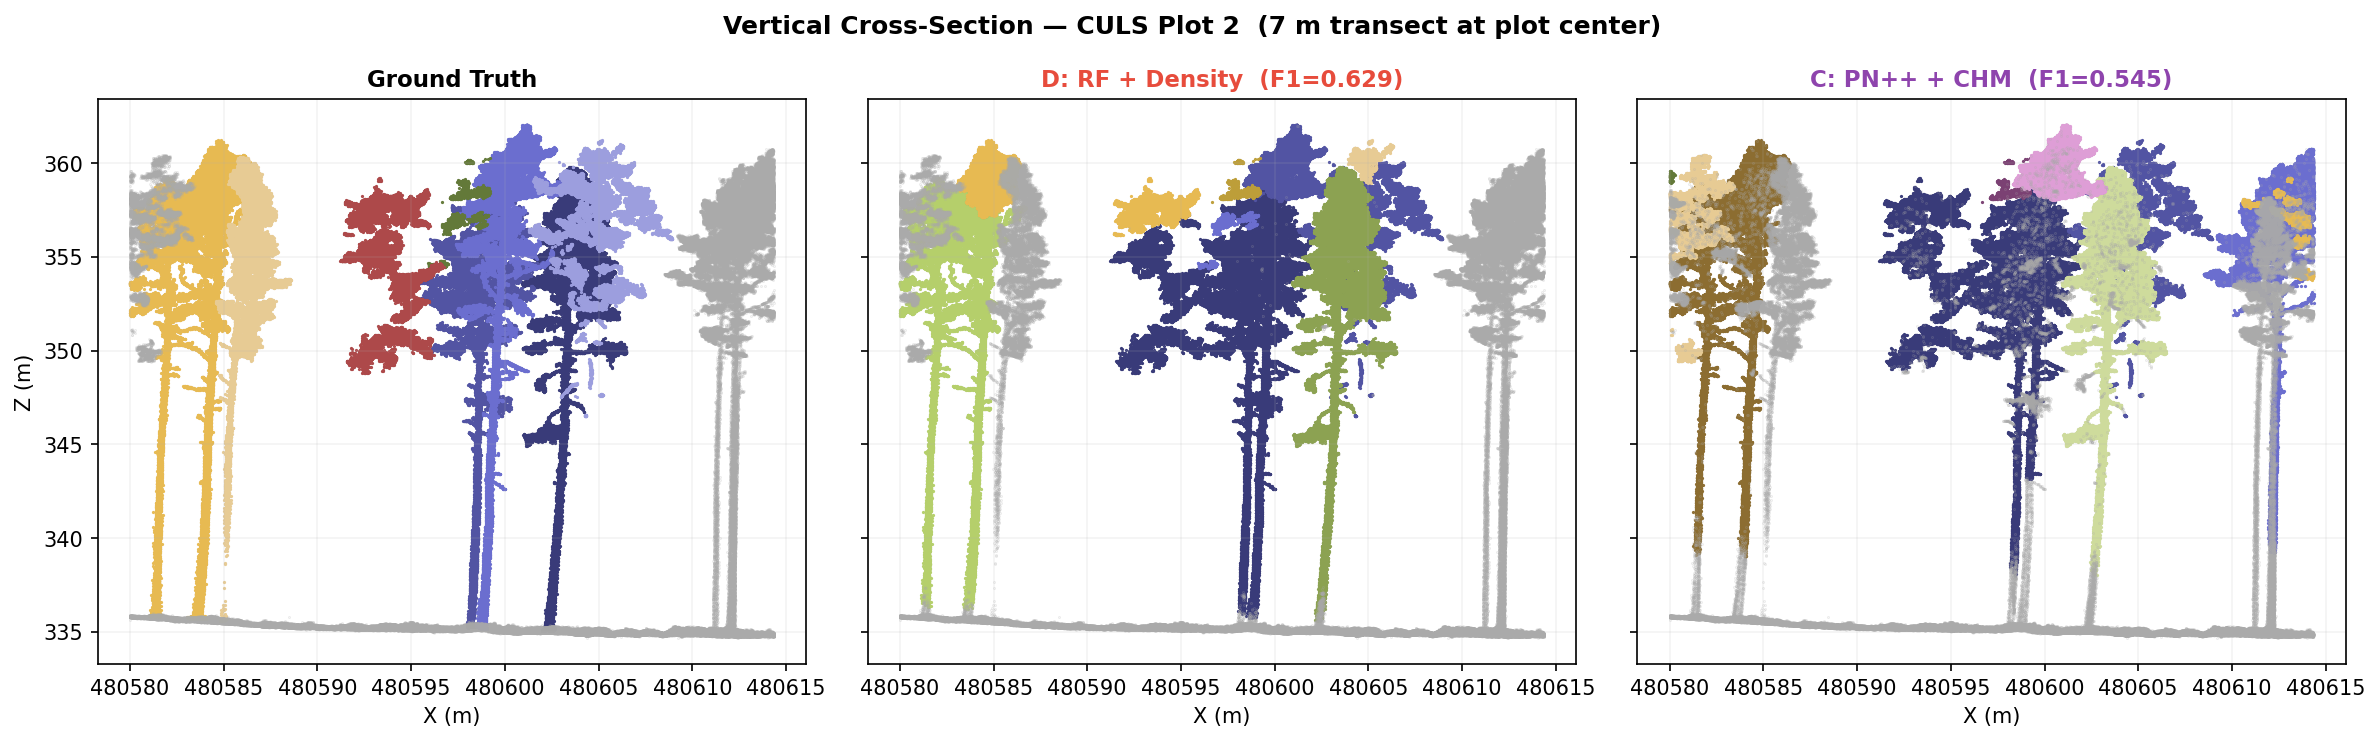
\includegraphics[width=\textwidth]{fig_v5_vertical_profile}
\caption{Vertical profile (7\,m) in CULS~Plot~2. Pipeline~D (center) correctly separates trees using volumetric fill; PointNet++ + CHM (right) confuses shared trunks.}\label{fig:vprofile}
\end{figure}

The central finding (Fig.~\ref{fig:decoupling}) is that near-perfect semantics (tree~IoU~$>$~0.97) do not translate into proportional instance quality (peak F1 0.209). The limiting factor is the ability of Watershed~3D to generate correct seeds and separate adjacent crowns. The factorial analysis confirms that the most productive investment in a two-stage ITS pipeline is not improving semantics --- where RF already excels --- but improving the instance segmenter. The effect is site-dependent: at CULS (separated crowns), RF+CHM reaches F1\,=\,0.811 and density seeding adds no substantial gain; at NIBIO, RMIT, and TUWIEN, where crowns overlap, CHM fails systematically and density seeding is required to obtain non-trivial performance.

\subsection{RF vs.\ PointNet++: GPU-Free Viability and Generalization}

RF outperforms PointNet++ in all seeding combinations. This advantage is not explained by superior semantics (tree~IoU gap $<$~1\,pp), but by better interaction with the segmenter: RF errors are crown-edge false positives, while PointNet++ generates isolated ground false positives that produce spurious seeds. Furthermore, RF trains and infers on CPU (${\sim}16$\,min) without requiring a GPU.

PointNet++ exhibits a severe performance drop at RMIT and TUWIEN (F1\,=\,0.000 with CHM), because its global subsampling of $8{,}192$ points does not adequately capture sites with densities and morphologies that differ from the training data (dominated by NIBIO boreal forest). RF, operating on local features, generalizes better across diverse forest types.

\subsection{Limitations}

The test set comprises 11~plots and 323~GT trees, which introduces per-site variance in estimates (especially CULS with 20~trees and TUWIEN with 35). PointNet++ is evaluated with a single hyperparameter configuration; an exhaustive search could improve its performance. The bottleneck conclusions are specific to the volumetric Watershed~3D; other segmenters (TreeLearn~\cite{henrich2024}, SegmentAnyTree~\cite{wielgosz2024}) could show a different relationship. Results are specific to ULS data ($454$--$10{,}156$~pts/m$^2$); transfer to conventional ALS is not guaranteed.

%% ================================================================
%%  8. CONCLUSIONS
%% ================================================================
\section{Conclusions}\label{sec:conclusions}

Using a $3 \times 2$ factorial design on FOR-instance~V1, we demonstrate that: (1)~the instance segmenter, not semantic preprocessing, is the main bottleneck of the ITS pipeline; (2)~Random Forest with geometric features outperforms PointNet++ MSG in all evaluated combinations, without requiring a GPU; and (3)~crown-density seeding consistently improves over CHM seeding (+47\% for RF, +74\% for PointNet++), being especially effective in dense forests with uniform canopy height.

The RF + Watershed~3D Density combination achieves the best instance F1 (0.209 on test), establishing a robust and efficient baseline. The gap between semantic and instance quality suggests that the most impactful improvements in ITS will come from segmenters capable of separating adjacent crowns in dense canopies --- through crown geometry priors, end-to-end segmenters, or better seeding strategies. Future work includes comparison with TreeLearn~\cite{henrich2024} and SegmentAnyTree~\cite{wielgosz2024}, extension to FOR-instanceV2~\cite{xiang2025}, and adaptive seeding strategies that combine CHM and density according to local height variability. Source code and reproduction scripts are available at \url{https://github.com/Cantuuuu/ITS-Pipeline-Comparison}.

%% ================================================================
%%  REFERENCES
%% ================================================================
\begin{thebibliography}{10}

\bibitem{puliti2023}
Puliti, S., et al.:
FOR-instance: a UAV laser scanning benchmark dataset for semantic and instance segmentation of individual trees.
arXiv preprint arXiv:2309.01279 (2023).
DOI: 10.5281/zenodo.8287792

\bibitem{qi2017}
Qi, C.R., Yi, L., Su, H., Guibas, L.J.:
PointNet++: Deep hierarchical feature learning on point sets in a metric space.
In: Advances in Neural Information Processing Systems (NeurIPS), pp.~5099--5108 (2017)

\bibitem{qi2016}
Qi, C.R., Su, H., Mo, K., Guibas, L.J.:
PointNet: Deep learning on point sets for 3D classification and segmentation.
In: IEEE Conference on Computer Vision and Pattern Recognition (CVPR), pp.~652--660 (2017)

\bibitem{yan2019pointnet2pytorch}
Yan, X.:
\texttt{Pointnet\_Pointnet2\_pytorch}: PyTorch implementation of PointNet and PointNet++.
GitHub repository, \url{https://github.com/yanx27/Pointnet_Pointnet2_pytorch} (2019). Accessed 2026-04

\bibitem{breiman2001}
Breiman, L.:
Random Forests.
Machine Learning \textbf{45}(1), 5--32 (2001)

\bibitem{weinstein2021}
Weinstein, B.G., Marconi, S., Bohlman, S., Zare, A., White, E.:
A benchmark dataset for canopy crown detection and delineation in co-registered airborne RGB, LiDAR and hyperspectral imagery from the National Ecological Observation Network.
PLOS Computational Biology \textbf{17}(7), e1009180 (2021).
DOI: 10.1371/journal.pcbi.1009180

\bibitem{silva2016}
Silva, C.A., Hudak, A.T., Vierling, L.A., et al.:
Imputation of individual longleaf pine (\emph{Pinus palustris} Mill.) tree attributes from field and LiDAR data.
Canadian Journal of Remote Sensing \textbf{42}(5), 554--573 (2016)

\bibitem{popescu2002}
Popescu, S.C., Wynne, R.H., Nelson, R.F.:
Estimating plot-level tree heights with lidar: local filtering with a canopy-height based variable window size.
Computers and Electronics in Agriculture \textbf{37}(1--3), 71--95 (2002)

\bibitem{dalponte2016}
Dalponte, M., Coomes, D.A.:
Tree-centric mapping of forest carbon density from airborne laser scanning and hyperspectral data.
Methods in Ecology and Evolution \textbf{7}(10), 1236--1245 (2016)

\bibitem{xiang2025}
Xiang, B., et al.:
ForestFormer3D: A unified framework for end-to-end segmentation of forest LiDAR 3D point clouds.
In: IEEE/CVF International Conference on Computer Vision (ICCV), Honolulu, Hawaii (2025).
arXiv:2506.16991

\bibitem{weinmann2015}
Weinmann, M., Jutzi, B., Hinz, S., Mallet, C.:
Semantic point cloud interpretation based on optimal neighborhoods, relevant features and efficient classifiers.
ISPRS Journal of Photogrammetry and Remote Sensing \textbf{105}, 286--304 (2015)

\bibitem{weinmann2017}
Weinmann, M., Jutzi, B., Mallet, C., Weinmann, M.:
Geometric features and their relevance for 3D point cloud classification.
ISPRS Annals of the Photogrammetry, Remote Sensing and Spatial Information Sciences \textbf{IV-1/W1}, 157--164 (2017)

\bibitem{henrich2024}
Henrich, J., et al.:
TreeLearn: A deep learning method for segmenting individual trees from ground-based LiDAR forest point clouds.
Ecological Informatics \textbf{84}, 102888 (2024).
DOI: 10.1016/j.ecoinf.2024.102888. arXiv:2309.08471

\bibitem{wielgosz2024}
Wielgosz, M., Puliti, S., Xiang, B., Schindler, K., Astrup, R.:
SegmentAnyTree: A sensor and platform agnostic deep learning model for tree segmentation using laser scanning data.
Remote Sensing of Environment \textbf{313}, 114367 (2024).
DOI: 10.1016/j.rse.2024.114367. arXiv:2401.15739

\end{thebibliography}

\end{document}
